\documentclass[10pt, a5paper]{article}
\usepackage{pdfpages}
\usepackage{parallel}
\usepackage[T2A]{fontenc}
\usepackage{ucs}
\usepackage[utf8x]{inputenc}
\usepackage[polish,english,russian]{babel}
\usepackage{hyperref}
\usepackage{rotating}
\usepackage[inner=2cm,top=1.8cm,outer=2cm,bottom=2.3cm,nohead]{geometry}
\usepackage{listings}
\usepackage{graphicx}
\usepackage{wrapfig}
\usepackage{longtable}
\usepackage{indentfirst}
\usepackage{array}
\newcolumntype{P}[1]{>{\raggedright\arraybackslash}p{#1}}
\frenchspacing
\usepackage{fixltx2e} %text sub- and superscripts
\usepackage{icomma} % коскі ў матэматычным рэжыме
\PreloadUnicodePage{4}

\newcommand{\longpage}{\enlargethispage{\baselineskip}}
\newcommand{\shortpage}{\enlargethispage{-\baselineskip}}

\def\switchlang#1{\expandafter\csname switchlang#1\endcsname}
\def\switchlangbe{
\let\saverefname=\refname%
\def\refname{Літаратура}%
\def\figurename{Іл.}%
}
\def\switchlangen{
\let\saverefname=\refname%
\def\refname{References}%
\def\figurename{Fig.}%
}
\def\switchlangru{
\let\saverefname=\refname%
\let\savefigurename=\figurename%
\def\refname{Литература}%
\def\figurename{Рис.}%
}

\hyphenation{admi-ni-stra-tive}
\hyphenation{ex-pe-ri-ence}
\hyphenation{fle-xi-bi-li-ty}
\hyphenation{Py-thon}
\hyphenation{ma-the-ma-ti-cal}
\hyphenation{re-ported}
\hyphenation{imp-le-menta-tions}
\hyphenation{pro-vides}
\hyphenation{en-gi-neering}
\hyphenation{com-pa-ti-bi-li-ty}
\hyphenation{im-pos-sible}
\hyphenation{desk-top}
\hyphenation{elec-tro-nic}
\hyphenation{com-pa-ny}
\hyphenation{de-ve-lop-ment}
\hyphenation{de-ve-loping}
\hyphenation{de-ve-lop}
\hyphenation{da-ta-ba-se}
\hyphenation{plat-forms}
\hyphenation{or-ga-ni-za-tion}
\hyphenation{pro-gramming}
\hyphenation{in-stru-ments}
\hyphenation{Li-nux}
\hyphenation{sour-ce}
\hyphenation{en-vi-ron-ment}
\hyphenation{Te-le-pathy}
\hyphenation{Li-nux-ov-ka}
\hyphenation{Open-BSD}
\hyphenation{Free-BSD}
\hyphenation{men-ti-on-ed}
\hyphenation{app-li-ca-tion}

\def\progref!#1!{\texttt{#1}}
\renewcommand{\arraystretch}{2} %Іначай формулы ў матрыцы зліпаюцца з лініямі
\usepackage{array}

\def\interview #1 (#2), #3, #4, #5\par{

\section[#1, #3, #4]{#1 -- #3, #4}
\def\qname{LVEE}
\def\aname{#1}
\def\q ##1\par{{\noindent \bf \qname: ##1 }\par}
\def\a{{\noindent \bf \aname: } \def\qname{L}\def\aname{#2}}
}

\def\interview* #1 (#2), #3, #4, #5\par{

\section*{#1\\{\small\rm #3, #4. #5}}

\def\qname{LVEE}
\def\aname{#1}
\def\q ##1\par{{\noindent \bf \qname: ##1 }\par}
\def\a{{\noindent \bf \aname: } \def\qname{L}\def\aname{#2}}
}

\begin{document}
\title{Flume и Morphlines "--- трансформация потоков данных без строчки кода}
\author{Денис Пынькин, Минск, Беларусь\footnote{\url{fannrm@gmail.com}, \url{http://lvee.org/en/abstracts/133}}}
\maketitle
\begin{abstract}
Apache Flume is a distributed, reliable, and available system for efficiently collecting, aggregating and moving large amounts of log data from many different sources to a centralized data store.
Morphlines is an open source framework that reduces the time and efforts necessary to build and change Hadoop ETL stream processing applications.
Combination of these technologies give a powerful tool for data stream transformation on distributed configurations without programming.
\end{abstract}
\subsection*{Введение}

Одним из столпов на которых стоят *nix системы является концепция «конвейеров» (pipeline) для обеспечения совместной работы множества программ. К сожалению возможности конвееров, без использования вспомогательных средств вроде netcat, ограничиваются пределами одного хоста и слабой параллелизацией данных. Даже классические задачи, например, сбор и обработка большого количества логов с фермы серверов становится головной болью администратора.

В то же время адепты Big Data активно развивают концепцию DataFlow, которая по сути является развитием все той же концепции конвейеров, но предназначена для организации управления большими потоками данных.

\subsection*{Apache Flume}

\begin{figure}[h!]
  \centering
  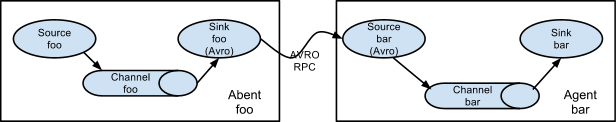
\includegraphics[scale=0.5]{21_2014_UserGuide_image03.png}
\end{figure}

Flume  \cite{Pynkin1} "--- это рапределенный, надежный сервис для эффективного сбора, агрегирования и передачи больших потоков данных. Простой и гибкий в настройке, Flume обладает очень архитектурой, позволяющей настроить буквально любой аспект поведения сервиса. Используется простая и легко расширяемая модель данных, что очень удобно для использования в аналитических сервисах.

Каждый агент Flume состоит из 3 составляющих:

\begin{itemize}
  \item source "--- источник данных, фактически сервис умеющий преобразовывать входные данные во внутреннее представление;
  \item channel "--- очередь сообщений, служащий связующим звеном между источником данных и выходом;
  \item sink "--- сервис умеющий преобразовать внутреннее представление данных в необходимое для потребителя.
\end{itemize}

Особую пикантность придает то, что помимо множества уже существующих «стандартных» компонентов, существует возможность легкого создания и использования любой из составляющих агента.

Каждая составляющая агента может состоять из одного или более компонентов, что превращает Flume в конструктор с возможностью построения любой топологии по передаче потоков данных.

\subsubsection*{Базовые блоки «конструктора»}

На данный момент существует несколько десятков стандартных компонентов и с каждым релизом их становится все больше:

\begin{itemize}
  \item Source "--- начиная от запуска любой утилиты, дающей вывод через stdout и заканчивая организацией полноценного сетевого сервиса, работающего с различными сетевыми протоколами: tcp, http, syslog, AVRO, Thrift и др.;
  \item Memory Channel "--- как in"=memory, для скорости, так и надежная очередь с записью промежуточных данных в файл или даже базу данных;
  \item Sink "--- от банальной записи в файл (организация логов) на локальной или кластерной файловой системе, до интеграции с другими агентами Flume или BigData системами.
\end{itemize}

Синтаксис файла конфигурации, описывающего агента очень прост и приспособлен для использования человеком:

\begin{verbatim}
# properties for sources 
<Agent>.sources.<Source>.<someProperty> = <someValue>
# properties for channels 
<Agent>.channel.<Channel>.<someProperty> = <someValue>
# properties for sinks 
<Agent>.sources.<Sink>.<someProperty> = <someValue> 
\end{verbatim}
\subsubsection*{Топология}

Возможность агентов Flume взаимодействовать между собой \linebreak позволяет создать действительно распределенную и, при необходимости, надежную сеть передачи потоков данных.

Так, например, с помощью Avro Sink и Avro Source очень легко реализовать агрегирование из нескольких источников в одну систему (топология «fan"=in»):


\begin{figure}[h!]
  \centering
  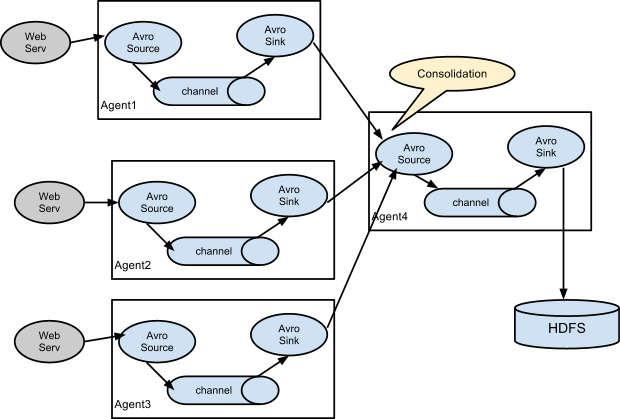
\includegraphics[scale=0.5]{21_2014_UserGuide_image02.png}
\end{figure}

Завязав несколько Sink на одну очередь можно легко добиться дробления одного потока данных на несколько более мелких (топология «fan"=out»).

А при использовании нескольких очередей можно добиться мультиплексирования (роутинга) отдельных записей «по условию», как это сделано в системах очередей сообщений:

\begin{figure}[h!]
  \centering
  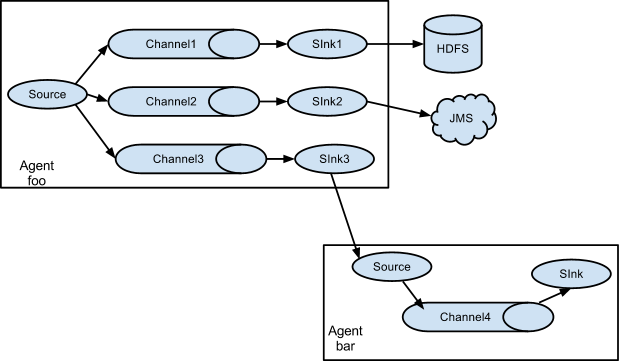
\includegraphics[scale=0.5]{21_2014_UserGuide_image01.png}
\end{figure}

\subsubsection*{Чудесное превращение Flume в ETL}

ETL \cite{Pynkin2} (от англ. Extract, Transform, Load — дословно «извлечение, преобразование, загрузка») — один из основных процессов в управлении хранилищами данных, который включает в себя:

\begin{itemize}
  \item извлечение данных из внешних источников;
  \item их трансформация и очистка, чтобы они соответствовали нуждам бизнес"=модели;
  \item и загрузка их в хранилище данных.
\end{itemize}

Если с Extract и Load у Flume все очевидно, то для Transform у Flume существует замечательный и мощнейщий механизм под названием «Interceptor», который позволяет производить преобразование данных в пределах каждой записи.
Как и для других элементов, для «Interceptor» существует несколько базовых механизмов, среди которых особняком стоит механизм Morphlines, позволяющий преобразовывать данные без строчки кода!

\subsection*{Morphlines}

Morphlines  \cite{Pynkin3} "--- это фреймфорк с открытым исходным кодом, разработанный как часть системы Cloudera Search. Основная цель создания Morphlines "--- быстрая разработка приложений для обработки потоков данных в Hadoop с последующей записью результатов в  Apache Solr, HBase, HDFS и прочие системы.

В лучших традициях «правила разделения» приведенным Эриком Реймондом в его бессмертной книге «Искусство программирования в UNIX», в Morphlines была заложена концепция управления с помощью данных "--- фактически конфигурационного файла, описывающего pipeline последовательных преобразований для записи данных:

\begin{figure}[h!]
  \centering
  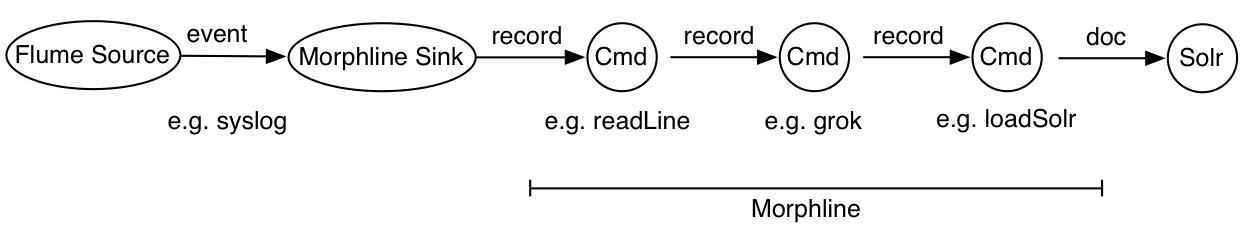
\includegraphics[scale=0.5]{21_2014_morphlines.jpg}
\end{figure}

Фреймворк получился настолько удачным, что он был выделен в отдельную часть, а также предусмотрены механизмы для встраивания в любое приложение написанное на Java.

\subsubsection*{Модель данных}

Концепция Morphlines предполагает, что данные поступают в виде бесконечного (или хотя бы достаточно большого) потока записей.

Центральной частью Morphlines является запись (Record), которая представляет собой набор именованных полей, причем каждое поле может содержать от одного и более значений. Поля записи могут использоваться как key"=value пары, так и выстраиваться в более сложные связи. Для упрощения можно рассматривать работу с записью, как работу с JSON"=объектом, поскольку поддерживаются все возможности по организации данных, которые предоставляются этой нотацией.

На самом деле все еще более интересно, поскольку в качестве значения для поля можно использовать любой объект Java.

\subsubsection*{Конфигурационный файл}

Конфигурационный файл представляет собой последователь- \linebreak ный список команд для преобразования данных, описанный в формате HOCON (Human Optimized Config Object Notation), кроме того предоставляются возможности бранчевания с помощью команд pipe, if и tryRules.

Список возможных команд преобразования чрезвычайно обширен \cite{Pynkin4}, но не ограничивается только предопределенными командами "--- достаточно легко можно написать свою реализацию недостающего функционала. Более того, с помощью команды «java» можно встраивать исходный код прямо в конфигурационный файл!

Чрезвычайно мощным инструментом является команда «grok» реализующая разбор любой текстовой строки с помощью регулярных выражений с использованием одноименного синтаксиса из пакета LogStash \cite{Pynkin5}. Особенно приятно то, что для отладки можно использовать онлайн дебаггер «Grok Debugger» \cite{Pynkin6}.

В онлайн-версии данных тезисов дополнительно рассмотрен подробный синтетический пример использования предлагаемой связки:  схема, собирающая статистику скачивания файлов со множества FTP"=серверов и сохраняющая ее в файл в формате JSON.

%\subsection*{Синтетический пример}
%
%Disclaimer: поскольку работающая система прикрыта завесой NDA, для примера был взят первый попавшийся работающий сервис "--- FTP"=сервер «vsftpd».
%
%В качестве примера разработаем систему, собирающую статистику скачивания файлов со множества FTP"=серверов и сохраняющую ее в файл в формате JSON, с указанием времени скачивания (в Unix time), имени файла, IP"=адреса клиента, а так же, в качестве бонуса, имени сервера с которого скачали этот файл.
%
%В логе vsftpd данная строка выглядит следующим образом:
%
%\begin{verbatim}
%Tue Jul 22 19:15:23 2014 [pid 9388] [vsftpd] OK DOWNLOAD: 
%Client "10.6.136.54", "/video/HighLoad master-class/out-
%1406031869.mkv", 189505527 bytes, 3909.30Kbyte/sec
%\end{verbatim}
%\subsubsection*{Конфигурационный файл для Flume}
%
%В примере описаны два агента:
%
%\begin{itemize}
%  \item vsftpd "--- для парсинга логов и отсылки данных на центральный сервер
%  \item collector "--- принимает данные от FTP"=серверов и складывает в файлы
%\end{itemize}
%
%\begin{verbatim}
%### Agent working on vsftpd node
%vsftpd.sources = logreader
%vsftpd.channels = mem-channel
%vsftpd.sinks = avro-out
%# default memory channel
%vsftpd.channels.mem-channel.type = memory
%# Read from log file
%vsftpd.sources.logreader.type = exec
%vsftpd.sources.logreader.command = tail -F /var/log/vsftp
%d.log
%vsftpd.sources.logreader.channels = mem-channel
%# expecting veeeeery loooong string
%vsftpd.sources.logreader.deserializer = LINE
%vsftpd.sources.logreader.deserializer.maxLineLength = 327
%68
%# set interceptor for converting string to AVRO
%vsftpd.sources.logreader.interceptors = morphline
%# morphline interceptor config
%vsftpd.sources.logreader.interceptors.morphline.type = or
%g.apache.flume.sink.solr.morphline.MorphlineInterceptor\$
%Builder
%vsftpd.sources.logreader.interceptors.morphline.morphline
%File = /tmp/flume/conf/morphlines.conf
%vsftpd.sources.logreader.interceptors.morphline.morphline
%Id = vsftpFileLog
%# sink stream over avro channel
%vsftpd.sinks.avro-out.type = avro
%vsftpd.sinks.avro-out.channel = mem-channel
%vsftpd.sinks.avro-out.hostname = 127.0.0.1
%vsftpd.sinks.avro-out.port = 5555
%
%### Logs collector agent
%collector.sources = avro-in
%collector.channels = mem-channel
%collector.sinks = file-out
%# get stream over avro channel
%collector.sources.avro-in.type = avro
%collector.sources.avro-in.channels = mem-channel
%collector.sources.avro-in.bind = 0.0.0.0
%collector.sources.avro-in.port = 5555
%# default memory channel
%collector.channels.mem-channel.type = memory
%# write stream to file every 5 minutes or 1000 events
%collector.sinks.file-out.type = file_roll
%collector.sinks.file-out.sink.rollInterval = 300
%collector.sinks.file-out.batchSize = 1000
%collector.sinks.file-out.sink.directory = /tmp/flume/log/
%collector.sinks.file-out.channel = mem-channel
%\end{verbatim}
%Для оптимизации необходимо «поиграться» с настройками, особенно каналов. Также необходимо проверить пути в конфигурационном файле и адаптировать их к своей системе.
%
%\subsubsection*{Файл преобразований Morphlines}
%
%Описание преобразований находится в комментариях к каждой из команд Morphlines.
%
%\begin{verbatim}
%morphlines: [
%  {
%    id: vsftpFileLog
%
%    importCommands: [ "org.kitesdk.**" ]
%
%    commands: [
%      { readLine { charset : UTF-8 } }
%
%      # Parse input string and extract fields:
%      # timestamp, ip, file, size
%      { grok {
%          dictionaryFiles : [ /tmp/flume/conf/grok ]
%	  dictionaryString : """
%	    TS %{DAY} %{MONTH} %{MONTHDAY} %{TIME} %{YEAR}
%	    PATH (?>/(?>[\w\s_%!$@:.,-]+|\\.)*)+
%          """
%          expressions : {
%            message : """%{TS:timestamp}.*Client "%{IP:ip}",
%             "%{PATH:file}", %{INT:size}.*"""
%          }
%      } }
%      # Convert input time from custom to Unixtime format
%      { convertTimestamp {
%          field : timestamp
%          inputFormats : [ "EEE MMM dd HH:mm:ss yyyy" ]
%          outputFormat : "unixTimeInSeconds"
%      } }
%      # Add name of host to field "server"
%      { addLocalHost {
%          field : server
%          useIP : false
%      } }
%      # Convert Morphline Record to AVRO-event according 
%      # schema
%      { toAvro { 
%        schemaString : """
%	{ "type": "record",
%	  "name": "ftpfile",
%	  "fields": [
%		{ "name": "timestamp", "type": "long",   "default": -1 },
%		{ "name": "server",    "type": "string", "default": "" },
%		{ "name": "ip",        "type": "string", "default": "" },
%		{ "name": "file",      "type": "string", "default": "" },
%		{ "name": "size",      "type": "long",   "default": -1 }
%        ]}
%
%        """
%      } }
%      # serialize the object
%      { writeAvroToByteArray: {
%        format: containerlessJSON
%      } }
%    ]
%  }
%]
%\end{verbatim}
%\subsubsection*{Запуск}
%
%Монитор лог"=файлов сервера:
%
%\begin{verbatim}
%flume-ng agent -n vsftpd -f /tmp/flume/conf/flume.propert\
%ies -C "/usr/lib/kite/*:/usr/lib/kite/lib/*"
%\end{verbatim}
%И «сервер» занимающийся сбором статистики и записью в файлы:
%
%\begin{verbatim}
%flume-ng agent -n collector -f /tmp/flume/conf/flume.prop\
%erties
%\end{verbatim}
\subsection*{Краткий вывод}

При совместном использовании Flume с поддержкой Morphlines можно организовать распределенную систему обработки потоковых данных почти любой сложности, буквально не написав ни строчки кода, что должно особенно понравится администраторам.

Также можно констатировать, что, не смотря на то, что оба инструмента написаны на Java, их архитектура отлично укладывается в принципы, декларируемые философией Unix, а использование близко к «классической» концепции pipeline.
\begin{thebibliography}{9}
\bibitem{Pynkin1} \url{http://flume.apache.org/FlumeUserGuide.html} 
\bibitem{Pynkin2} \url{https://ru.wikipedia.org/wiki/ETL} 
\bibitem{Pynkin3} \url{http://kitesdk.org/docs/current/kite-morphlines/index.html} 
\bibitem{Pynkin4} \url{http://kitesdk.org/docs/current/kite-morphlines/morphlinesReferenceGuide.html} 
\bibitem{Pynkin5} \url{http://logstash.net/docs/1.4.2/filters/grok} 
\bibitem{Pynkin6} \url{http://grokdebug.herokuapp.com/}
\end{thebibliography}
\end{document}
